
\section{Using Machine Learning to analyse Mass Spectrometer Data} \label{sec:Mars}

This section of this thesis are based on work carried out during a four-month period in 2024 during a research exchange and software acceleration program known as the Frontier Development Lab (FDL) hosted by the SETI Institute in partnership with the NASA Goddard Flight Center (GSFC). While this work may not seem to appear relevant to the rest of the work described in this thesis it is at its core related to SETI and radio astronomy data analysis. One of the main purposes of the program is to solve problems that may have stagnated in their respective field or just require more manpower. FDL brings together an array of researches at PhD and postdoc level from variouss backgrounds to bring new ideas from their own research, to a specific problem proposed by the funding body (in this case GSFC). The problems themselves require machine learning (ML) to solve, so each team is usually comprised of two ML experts, two science experts and a faculty or industry experts. Based in Silicon Valley there is also amble access to discuss the projects directly with the hardware providers, in the case of this project Google and NVIDIA. The data from mass spectrometers come in the same form as filterbank files, as  dynamic spectra. This is where the value of a radio astronomy background became evident. The exchange provided extensive experience in machine learning, GPU processing, cloud computing, and model optimisation. These skills formed the foundation for the machine learning techniques described earlier in this thesis, as well as several other projects currently in their preliminary stages that will be discussed in the next chapter.
The following work was carried out with equal contributions by Owen Johnson, Kanak Parmar, Arushi Saxena, Pugazhenthi Sivasankar and Robert Alvarez. The content presented in this section has been retained as closely as possible to the original wording of the associated NASA patent documentation, accompanying technical memorandum, and conference paper to preserve the technical accuracy and intent of the original work produced by the above authors. However, sections of the work that did not primarily constitute the thesis author's own contributions have been removed, and additional edits have been made to improve readability.


The search for life beyond Earth has been a driving force in planetary exploration, and Mars, with its intriguing geological features and past presence of liquid water, stands at the forefront of this quest. NASA's Curiosity rover, part of the Mars Science Laboratory (MSL) mission, has been instrumental in exploring the Red Planet's surface sinceit'ss landing in Gale Crater in August 2012 \citep{bogue2012mars, vasavada2022mission}. Among the suite of advanced scientific instruments aboard Curiosity, the Sample Analysis at Mars (SAM) instrument suite plays a pivotal role inunravellingg the mysteries of Martian geology and the planet's potential to support life \citep{mahaffy2012sample}.\\

SAM's primary mission is to analyze soil and rock samples for organic compounds and other volatile elements that are essential indicators of past or present life. By identifying a broad range of chemical signatures, SAM provides critical insights into the bio-chemical processes that have shaped Mars over billions of years. This instrument suite combines gas chromatography (GC), mass spectrometry (MS), and tunable laser spectroscopy (TLS)to conduct a comprehensive analysis of Martian samples, making it one of the most sophisticated laboratories ever sent to another planet.\\ 

These sample analyses provide valuable insights into the presence of key chemical compounds in the Martian crust, such as sulfates, water-bearing minerals, organics, and chlorides. This information can shed light on Mars' geochemical evolution and its potential for habitability. However, to conduct these analyses, experimental data must be sent to scientists on Earth through NASA's Deep Space Network (DSN) for review and interpretation \citep{sarkar2011survey}. Given the rover's limited operational time on Mars, there are two main challenges for future missions. The first is the latency and limited bandwidth of data transmission, and the second is the time required to analyze the data for various chemical compounds to determine the rover's next operations and desired analyses. \\

As a first-step to address these long-term challenges, this work explores machine learning (ML) and data science techniques to enhance the analysis of SAM datasets, particularly mass spectrometry data, to support scientists’ decision-making process during missions operations. The goal is to make science operations faster and more efficient, and ultimately maximize missions’ scientific returns, especially for missions to the outer solar system that will face more severe communication and resource limitations than missions to Mars. The available data is first explored followed by a brief discussion on the data cleaning and augmentation. Various ML techniques suitable for the processed data are then investigated. Using the best-fitting ML models, the performance metrics for each of the classified chemical signatures are quantified. Finally, a roadmap for the development of an in-situ classification model is discussed.  \\


As a first-step to address these long-term challenges, this work explores machine learning (ML) and data science techniques to enhance the analysis of SAM datasets, particularly mass spectrometry data, to support scientists’ decision-making process during missions operations. The goal is to make science operations faster and more efficient, and ultimately maximize missions’ scientific returns, especially for missions to the outer solar system that will face more severe communication and resource limitations than missions to Mars. The available data is first explored followed by a brief discussion on the data cleaning and augmentation. Various ML techniques suitable for the processed data are then investigated. Using the best-fitting ML models, the performance metrics for each of the classified chemical signatures are quantified. Finally, a roadmap for the development of an in-situ classification model is discussed.

\subsection{Context and Related Work}

This research concentrates primarily on exploring how leveraging ML and data science can aid and enhance the analysis of Martian surface samples, with the ultimate goal of improving efficiency of identifying chemical compounds present in the samples. The data used in this challenge is centered around the SAM instrument on NASA’s Curiosity rover and similar commercially available instruments.

The secondary output of this research is to explore how viable it would be to develop a robust ML pipeline that could be generalized to other scientific and exploratory missions, particularly in situations where data needs to be analyzed in-situ without human supervision. These goals are directly reflected by the motivations listed in the previous section.

The core of this research focuses on the development of tailored ML models to process and analyze Mass Spectrometry (MS) data produced by SAM (and other instruments) using similar logic as a scientist would. These models need to identify chemical signatures rapidly and correctly in collected samples on the Martian surface. These models are intended to act as a proof of concept for in-situ analysis on mass spectrometer instruments onboard future missions.

Before this, several projects have been completed to explore these objectives. Most notably, two challenges, organized and funded by NASA, were conducted before this project. The first challenge utilized datasets from Evolved Gas Analysis Mass Spectrometry (EGAMS) commercial instruments located at the NASA’s Goddard Space Flight Center (GSGFC) and Johnson Space Center (JSC) and flight-like data coming from the SAM testbed instrument located at NASA GSFC. The second challenge utilized Gas Chromatography Mass Spectrometry (GCMS) data from commercial spectrometers located at NASA GSFC. Two performance metrics were used to assess the performance: i) log loss for which the desired value should be as close to zero as possible, ii) micro-averaged average precision for which the desired value should be as close to one as possible. The first prize winner of the EGAMS challenge had an overall log loss score of 0.0920 and a micro-averaged average precision value of 0.9483. The overall log loss score of the first prize winner of the GCMS challenge was 0.1443 and the micro-averaged average precision was 0.8069. More details can be found in  \cite{da2024leveraging}. The main difference between this project and these previous challenges is the inclusion of the Mars data sent by the rover Curiosity and archived on the NASA Planetary Data System (PDS) website.

\subsection{Mass Spectrometry}

Mass spectrometry is a form of analysis used to identify and quantify the chemical composition of a sample by measuring the mass-to-charge (m/z) ratio of its ions. This process involves ionizing the chemical compounds (samples) to generate ions. The generated ions are then filtered based on their mass and their charge by using magnetic and electric fields. By detecting the relative abundance of these ions, mass spectrometers can provide detailed information about the molecular structure, composition, and purity of a sample. This technique is widely used in various fields, including chemistry, biology, environmental science, and planetary exploration, for its precision and ability to analyse complex mixtures.

\begin{figure}[h]
    \centering
    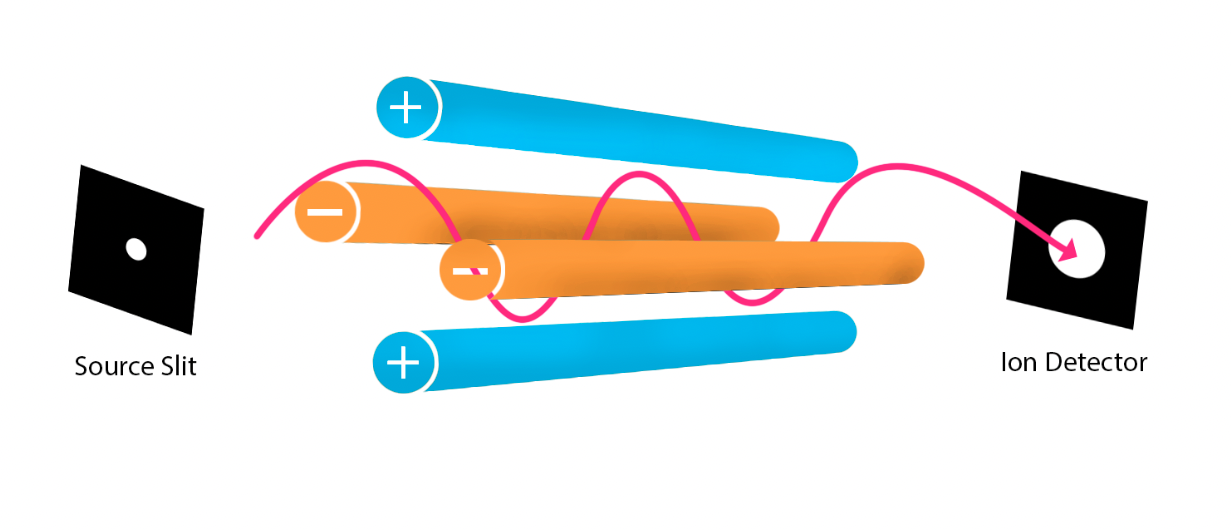
\includegraphics[width=0.8\linewidth]{chapter8/figs/Diagram/MS .png}
    \caption{Simplified overview of time-of-flight quadrupole mass spectrometer. Ions are accelerated through a source slit and deflected by a series of electric fields before reaching the ion detector, allowing for mass analysis based on their time of flight. Resonant ions, matching the frequency of the applied field, experience enhanced deflection and can be selectively detected.}
    \label{fig:MS}
\end{figure}

The data used in this challenge uses Time-of-Flight Mass Spectrometer (TOF-MS) as its end product for collecting data. A simplified overview can be seen in \cref{fig:MS}. Radio Frequency (RF) fields are used in manipulation and analysis of ions. RF fields are typically applied to quadrupole ion guides within the spectrometer, creating oscillating electric fields that can trap or filter ions based on their mass-to-charge ratio (m/z). These fields can also be used to excite ions into resonance, which causes them to oscillate with greater amplitude. When ions are resonant with the applied RF frequency, they undergo increased deflection, allowing for the selective passage or detection of specific ion species. This selective control is essential for enhancing the resolution and sensitivity of the mass spectrometer. The SAM instrument sweeps through varying RFs to detect m/z from 0 up to 500.

\subsubsection{Sample Analysis at Mars (SAM) Instrument Suite}

As previously mentioned, this challenge utilizes SAM instrument suite data. Below is a brief yet non-exhaustive overview\footnote{For a comprehensive review, see \cite{SAMPAPER_2012}} of the SAM instrument suite onboard the Curiosity rover. SAM’s primary function is to identify a range of primarily carbon-containing compounds. SAM’s capabilities to analyze samples can be summarized in three main stages. These stages involve sophisticated analytical techniques and consist of gas chromatography, mass spectrometry, and tunable laser spectroscopy.

\textbf{Sample Collection and Delivery:} When a suitable target is identified, Curiosity’s robotic arm collects a sample using either its scoop or drill, depending on the nature of the target material. The collected sample is then carefully portioned and delivered to SAM’s sample inlet tubes, ensuring that an adequate amount is available for subsequent analysis.

\textbf{Sample Processing and Analysis:} Upon receiving the sample, SAM employs a suite of analytical techniques to investigate its composition - gas chromatography, mass spectrometry, and tunable laser spectroscopy. Initially, the sample is heated in a quartz oven to release gases, which are analyzed to identify the presence of organic compounds and other volatile substances. Evolved Gas Analysis (EGA) analyzes the resulting gases from ablation. If Gas chromatography (GC) is being used, it then separates the different components of the gas mixture. Each method (EGA and GC) is subsequently fed into the mass spectrometer (MS) for molecular structure and composition analysis. Concurrently, the tunable laser spectrometer measures the concentrations of specific gases, such as methane, carbon dioxide, and water vapor, with high precision.

\textbf{Data Transmission and Analysis:} After the analysis is completed, the results are transmitted back to Earth, where scientists interpret the data to understand the chemical and mineralogical composition of the Martian samples. This information is crucial in assessing whether the sampled rocks and soil contain organic molecules key building blocks of life and in evaluating the past habitability of Mars.

 \begin{figure}
     \centering
     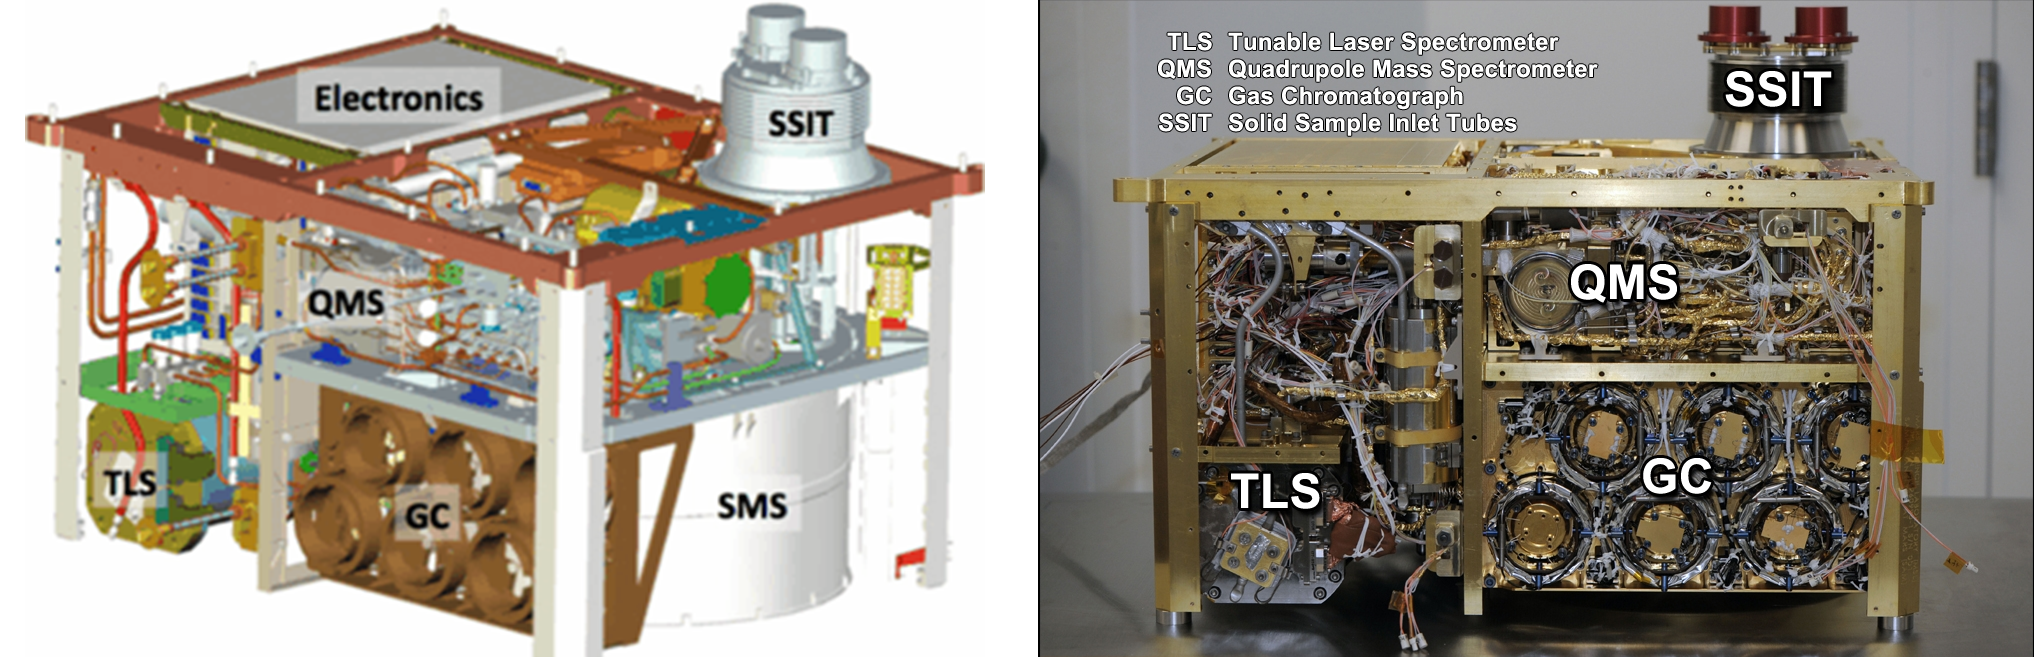
\includegraphics[width=0.9\linewidth]{chapter8/figs/Diagram/SAM-cross-section.png}
     \caption{Overview of the SAM instrument. Adapted from \citep{mahaffy2012sample}}
 \end{figure}


\subsection{Evoled Gas Analysis}

The Evolved Gas Analysis Mass Spectrometry (EGAMS) on SAM is designed to analyse gases released from Martian soil and rock samples when heated to high temperatures. An example of the data produced from EGAMS can be seen in \cref{fig:EGAMS-example}.

\begin{landscape}

\begin{figure}[p]
    \centering
    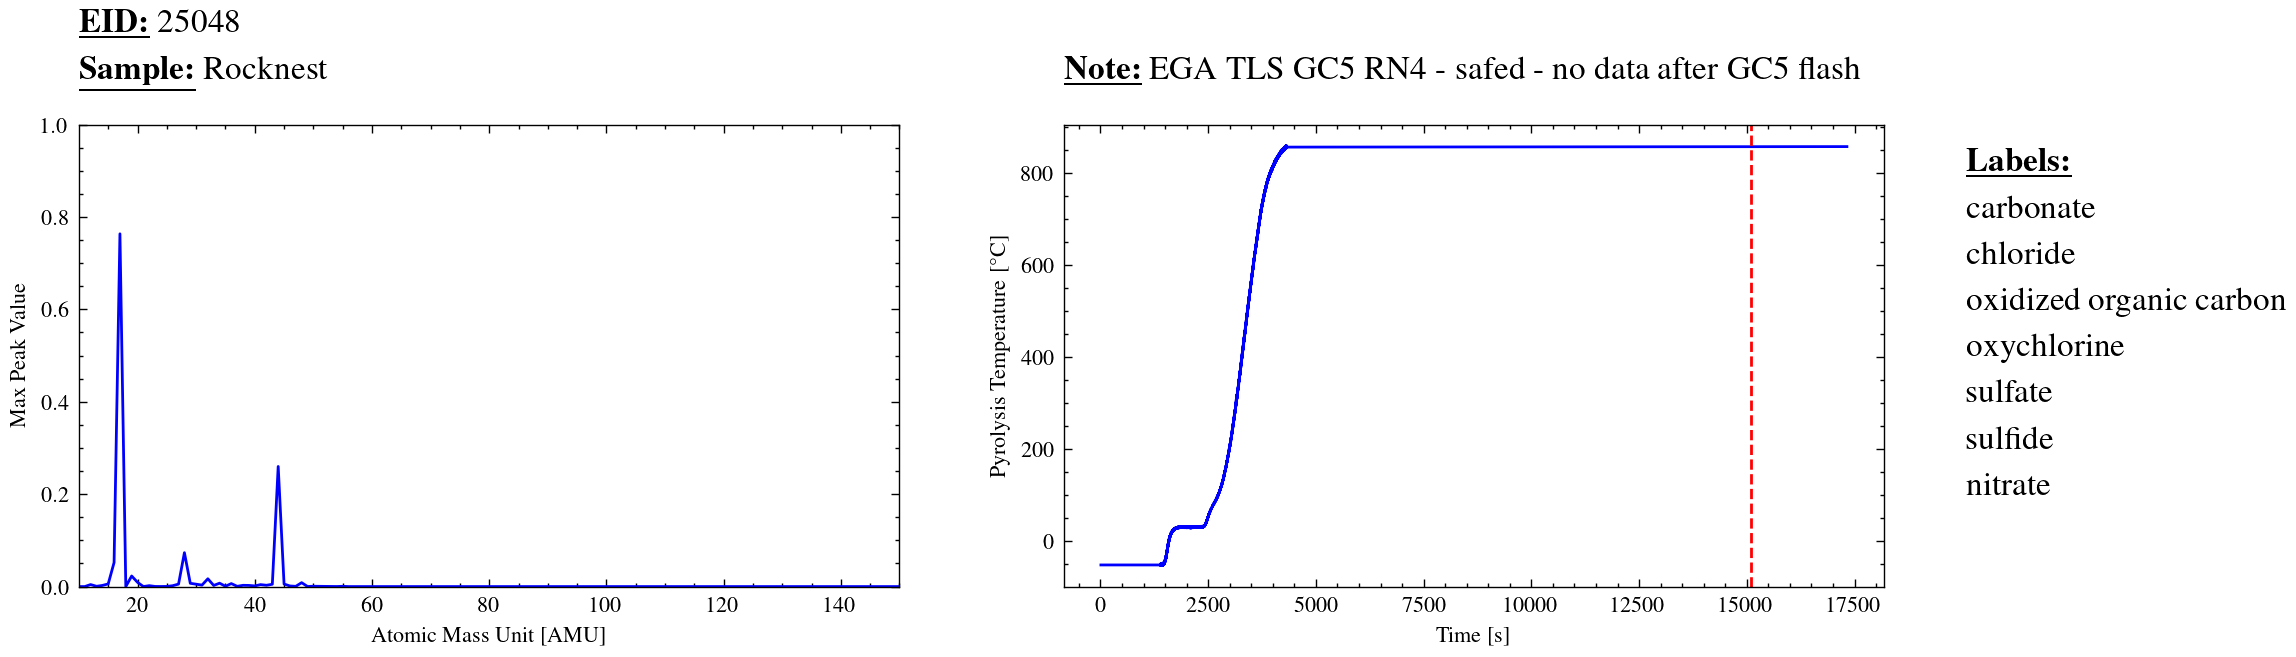
\includegraphics[width=0.99\linewidth]{chapter8/figs/25048_1725.png}
    \caption{Example of EGAMS data from SAM. The left panel shows atomic mass unit (AMU) against the normalized abundance. The right panel shows the pyrolysis (oven) temperature against run time. The hashed red line represents the time and temperature sample currently being shown. Labels assigned by scientists along with metadata associated with the specific sample are also shown.}
    \label{fig:EGAMS-example}
\end{figure}

\end{landscape}

As each sample is vaporized, a mass spectrum is recorded. Thus, for each studied sample there are hundreds of mass spectra. To visualize this, imagine that each sample run is a video that plays in time. Each frame of the video contains a mass spectrum. Counts per second on the y-axis and the mass-to-charge ratio or m/z values on the x-axis, the time and temperature are both intrinsically linked as the oven heats up over time. These values are represented by the number of each frame. An illustrative example of this can be seen in \cref{fig:data-cube-example}. 

\begin{figure}[h]
    \centering
    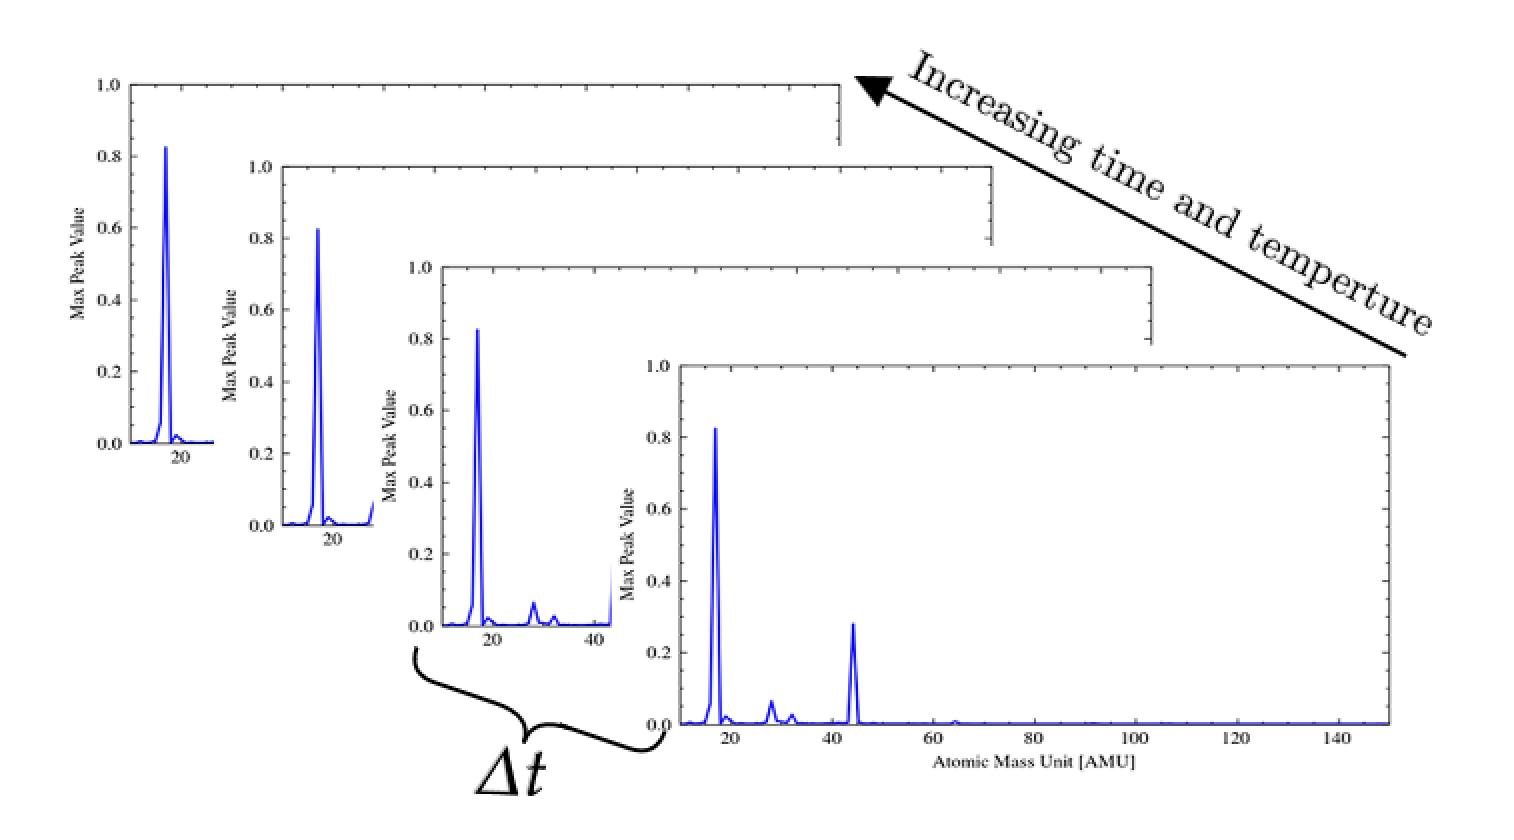
\includegraphics[width=0.8\linewidth]{chapter8/figs/data-cube-example.png}
    \caption{Multiple mass spectra with each being associated with a specific time and temperature.}
    \label{fig:data-cube-example}
\end{figure}


\subsubsection{SAM EGAMS Data}

The EGAMS data from Mars has some slight data cleaning applied to make the data more usable. This comes in the form of cropping the AMU ranges in the dataset. The Mars PDS data is cropped from 10 to 150 values. The reason 10 is used opposed to 0 is due to the presence of Helium (m/z $\approx$ 4 AMU) as the main gas carrier which makes it the most dominant peak in each of the collected samples. It is removed to better highlight variations seen throughout each sample run. Even though the mass spectrometer can cover up to m/z values of 533, it is generally cut at m/z = 150. The reason for this is because of the expected m/z values that a surface sample would produce as outlined in \cite{2015JGRE..120..495F}.


\subsubsection{Commercial EGAMS Data}

The instrument suite in SAM is based on other commercial MS instruments used at the Planetary Environments Laboratory (PEL) at NASA’s GSFC and JSC centers. Like SAM, these commercial instruments heat the sample over time, and the released gas ions are analysed to identify the chemical signatures in the sample by the end of the run, though all labels appear at the end of the run instead of at each image, as would be preferable for an ML model. Due to the controlled conditions of these commercial instruments, we have many more sample runs available — approximately 40 times more than what was provided from the SAM instrument on Mars. Additionally, the time-temperature relationship for commercial sample runs is systematic (see Fig. \ref{fig:commerical-data}), ensuring that the provided data is generally clean, with exceptions for a few samples that had excessive noise, negative abundance values, or fewer than five data points.


\begin{landscape}
\begin{figure}[p]
    \centering
    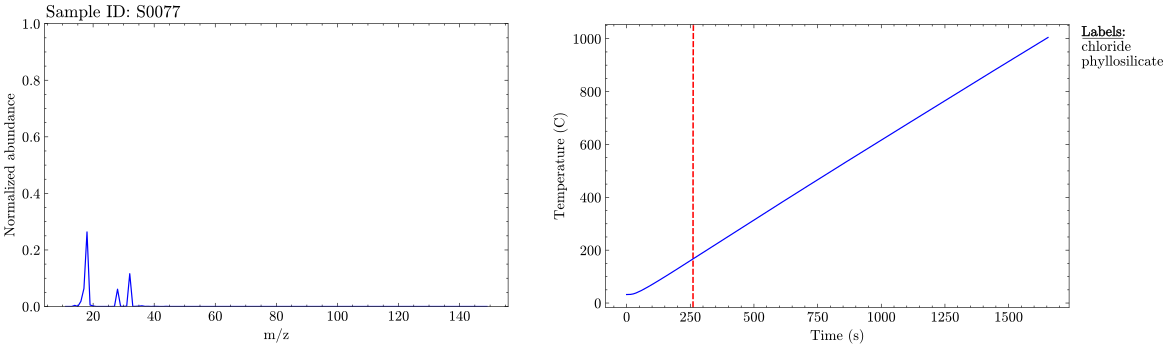
\includegraphics[width=0.99\linewidth]{chapter8/figs/commercial.png}
    \caption{Example of a sample run on a commercial mass spectrometer. The abundance across each sample run is normalized. The spectrum at a particular time is shown on the left for a given sample run as temperature increases with time following the distribution shown on the right. The dashed red line represents the time and temperature sample currently being shown}
    \label{fig:commerical-data}
\end{figure}
\end{landscape}

\subsubsection{Labeled Data}

To facilitate the use of the Mars and commercial datasets for ML and data science purposes, subject-matter experts labeled the datasets over a course of a year during weekly workshops. These labels were assigned based on the peaks in m/z values observed as a function of temperature. These labels were then assigned specific mineral classes which are listed in \cref{tab:label-comparison}.

However, in collecting the datasets, we observed insufficient overlap between the labels used for commercial and SAM datasets. Specifically, we identified a small subset of labels that were present in one dataset but not in the other. To address the lack of overlap, it was recommended by SAM scientists to unify the labels, using "Oxalate" in the commercial data interchangeably with "Oxidized organic compound" from the Mars dataset. Additionally, labels such as "Amorphous" and "Basalt" were disregarded, as they represent broader categories—non-crystalline compounds and rock types, respectively—rather than specific chemical entities. We keep all samples containing "Nitrate" in the Mars data and split them into roughly equal numbers for training and test sets (see \cref{sec:data_outputs}). This careful curation of labels ensures that the datasets are compatible for training ML models on the same labels for the two datasets.

\begin{table}[h]
    \centering
    \begin{tabular}{|p{25mm}|p{25mm}|}
        \hline
        \multicolumn{2}{|c|}{\textbf{Common}} \\
        \hline
        \multicolumn{2}{|c|}{Carbonate} \\
        \multicolumn{2}{|c|}{Chloride} \\
        \multicolumn{2}{|c|}{Iron-oxide} \\
        \multicolumn{2}{|c|}{Oxychlorine} \\
        \multicolumn{2}{|c|}{Phyllosilicate} \\
        \multicolumn{2}{|c|}{Silicate} \\
        \multicolumn{2}{|c|}{Sulfate} \\
        \multicolumn{2}{|c|}{Sulfide} \\
        \hline
        \multicolumn{2}{|c|}{\textbf{Uncommon}} \\
        \hline
        \textit{Mars} & \textit{Commercial} \\
        \hline
        Amorphous  & Basalt \\ 
        Oxidised organic compound & Oxalate \\
        Nitrate &  \\ 
        \hline
    \end{tabular}
    \caption{Label comparison between data from SAM's EGA and commercial instruments.}
    \label{tab:label-comparison}
\end{table}

\subsection{Data Augmentation}

The data provided from both the commercial and SAM instruments needed to be augmented to efficiently develop and train ML models. To begin with, we had 1,028 samples in the commercial dataset and 27 samples from the Mars PDS data, amounting to a total of 1055 samples (Table 4) which were not sufficient for training an image-based ML classifier. In general, for image-based classification problems, augmentation techniques such as rotating the image, horizontal and/or vertical flipping of the image, adding noise to the image and using a grey scale of the image are usually implemented to increase the amount of data used in training. Moreover, techniques such as flipping, down-sampling, inclusion of slope have been used to augment sequential data represented in time domain \cite{wen2020time}. Representing the sequential data in time-frequency domain, techniques such as amplitude adjusted Fourier transform (AAFT) and iterated AAFT (IAAFT) can be used \cite{lee2019surrogate}. However, many such techniques cannot be directly used for this mass spectrometry dataset. Care must be taken to ensure that the chemical information embedded in the numeric data of a sample should not be distorted too much during the data augmentation process, otherwise we risk losing the scientific accuracy of the data.
A single sample from the commercial and Mars PDS EGAMS data consists of four features: time, pyrolysis temperature, mass over charge (m/z), and intensity/counts. After considering the data representations from previous challenges, we chose to represent the outcomes of an EGAMS experiment as m/z vs intensity. This would result in a sequence of spectra where each spectrum is defined as a continuous stream of m/z (vs) intensity values with m/z column sorted in ascending order. This sequence of spectra implicitly includes the time and pyrolysis temperature information. The data augmentation methods were chosen to ensure the highest scientific accuracy, while still providing enough variability for the ML algorithm(s) to train on.
Before the data augmentation, both the commercial and Mars PDS data undergo pre-processing steps which facilitate the identification process of the compounds present in the sample. The first step in pre-processing is to remove the signal/intensity/abundance corresponding to m/z = 4 from the numeric data, corresponding to the Helium peak. Indeed, Helium, as an inert carrier gas, is used in the EGAMS experiments. Its peak is stronger by several orders of magnitude than all other species registered by the detector.
Next, all the abundance values corresponding to fractional m/z values (i.e., m/z = 4.5, 6.7, etc.) are removed as they could represent partially ionized species or isotopes which are not of primary interest to the scientists. Furthermore, the abundance values corresponding to m/z > 100 are also removed as they are due to heavier elements that are of less scientific significance when it comes to supporting life on other planets such as Mars. Finally, any background noise present is also removed. Outcomes of this preprocessing sequence are shown in \cref{fig:data-preprocess}. Each basic data augmentation type is applied to all the spectra present in an experiment. The pre-processed data is then subject to the following 6 basic data augmentation techniques:

\begin{enumerate}
    \item Shift: In each spectrum of a given sample, all the intensity values are shifted in one direction along the x-axis by a small amount defined by the shift parameter shown in the \cref{table:data-aug-para}. 

    \item Random shift: In each spectrum of a given sample, the peak indices are extracted. Out of these, a percentage of peak indices are chosen at random and shifted in one direction along the x-axis. The percentage of peak indices chosen depends on the value of the percentage of random peaks to shift (\cref{table:data-aug-para}). The degree of shift is given by the shift parameter from the same table. This value is in a small m/z range in order to keep the scientific accuracy of the mass spectrum.

    \item Randomized intensity variation: In each spectrum, $\sim 70\%$ of the data points are randomly selected and the intensity of each of the chosen points is modified by a small percentage value drawn at random from a uniform distribution with lower bound at zero and upper bound given by the intensity variation parameter (\cref{table:data-aug-para})

    \item White noise: A uniformly distributed background noise is added to each mass spectrum. The standard deviation of the noise is indicated in \cref{table:data-aug-para}.

    \item Gaussian noise: A zero mean Gaussian noise with a standard deviation of 0.05 is added to each mass spectrum (\cref{table:data-aug-para}).

    % \item Peak stretching: The highest peak of each spectrum is identified, and peaks on either sides of this highest peak are stretched to an extent defined by the stretch parameter value provided in Table \ref{table:data augmentation parameters}.

    \item Peak stretching: The highest peak of each spectrum is identified and stretched on either side to an extent defined by the stretch parameter value provided in \cref{table:data-aug-para}
\end{enumerate}

\begin{table}[h!]
\centering
\begin{tabular}{||c c||} 
 \hline
 \textbf{Parameter} & \textbf{Value }\\ [0.5ex] 
 \hline\hline
 shift parameter & 2 m/z \\ 
 Percentage of random peaks to shift  & 50\% \\
 Intensity variation  & 30\%\\
 standard deviation of the noise  & 0.05 \\
 stretch parameter value & 5 m/z \\ 
 [1ex] 
 \hline
\end{tabular}
\caption{Parameters for meaningful data augmentation}
\label{table:data-aug-para}
\end{table}

Using these 6 basic data augmentations, combinatorial augmentations can be performed in the following ways: $6C_2\,+\,6C_3\,+\,6C_4\,+\,6C_5\,+\,6C_5\,+\,6C_6$. 
This produces additional 57 combinatorial data augmentations (\cref{table:data-aug-comb}).
Including the 57 combinatorial data augmentations, 6 base data augmentations and the original data, each sample along with its label appears 64 times in the data set (Table \ref{table: Comparison of the number of samples in the original and augmented mass spectrometer data}).
After the augmentation, both the original and augmented data are normalized so that the intensity varies between 0 and 1 which facilitates the learning process of the ML algorithms.
Figure \ref{fig:data-aug} shows the 6 basic data augmentations while a single combination out of the 57 combinatorial data augmentations is depicted in Figure \ref{fig:data-aug-comb}.

\begin{table}[h!]
\centering
\begin{tabular}{||c|c|c||} 
 \hline
 \textbf{Augmentation combination} & \textbf{Amount} & \textbf{Examples}\\ [0.5ex] 
 \hline\hline
 $6C_2$ & 15 & Base 1 + Base 2, Base 1 + Base 3, ... \\ 
$6C_3$ & 20 & Base 1 + Base 2 + Base 3, Base 1 + Base 3 + Base 4, ... \\
$6C_4$ & 15 & Base 1 + Base 2 + Base 3 + Base 4, ... \\
$6C_5$ & 6 & Base 1 + Base 2 + Base 3 + Base 4 + Base 5, ... \\
 $6C_6$ & 1 & Base 1 + Base 2 + Base 4 + Base 5 + Base 6 \\
  Total & 57 & Not applicable \\ 
 [1ex] 
 \hline
\end{tabular}
\caption{Split up of combinatorial data augmentations}
\label{table:data-aug-comb}
\end{table}

The data augmentation is applied to each spectrum and the process is repeated for all the spectra in a sample.

\begin{figure}[h]
    \centering
    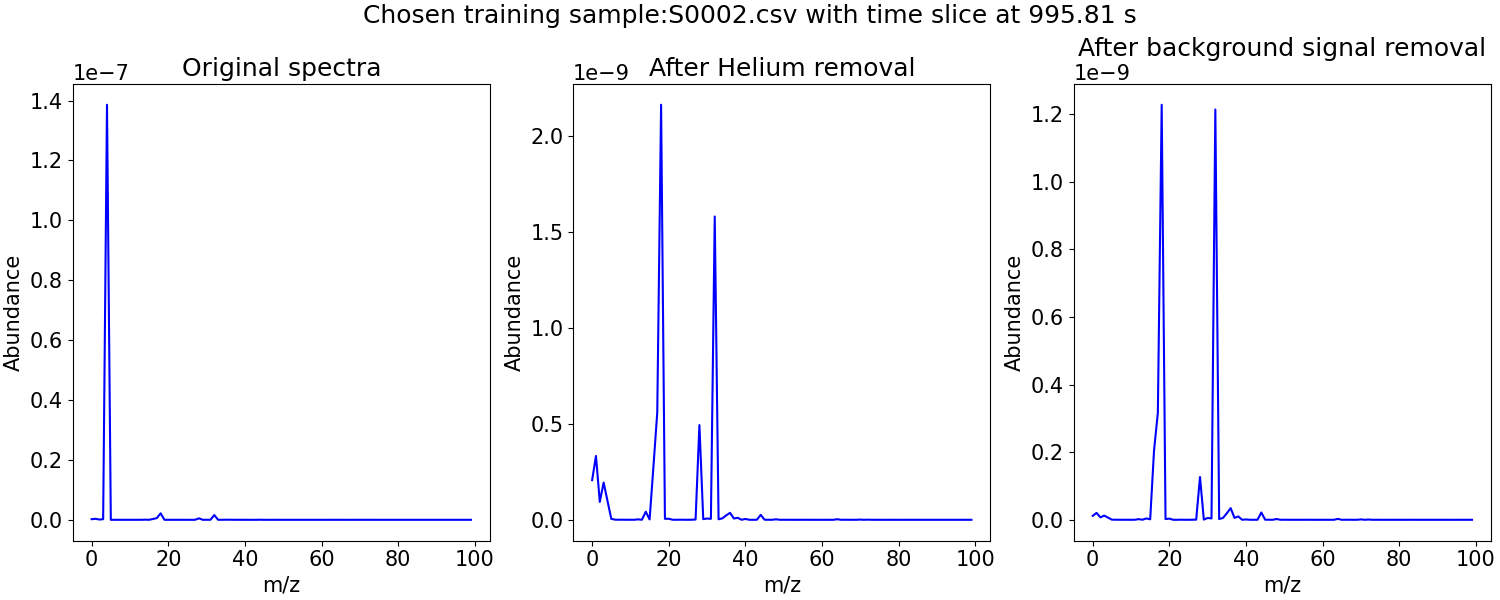
\includegraphics[width=1\linewidth]{chapter8/figs/data_preprocess.png}
    \caption{Stages of pre-processing mass spectrometry data in the m/z (vs) abundance representation.}
    \label{fig:data-preprocess}
\end{figure}

\begin{figure}[h]
    \centering
    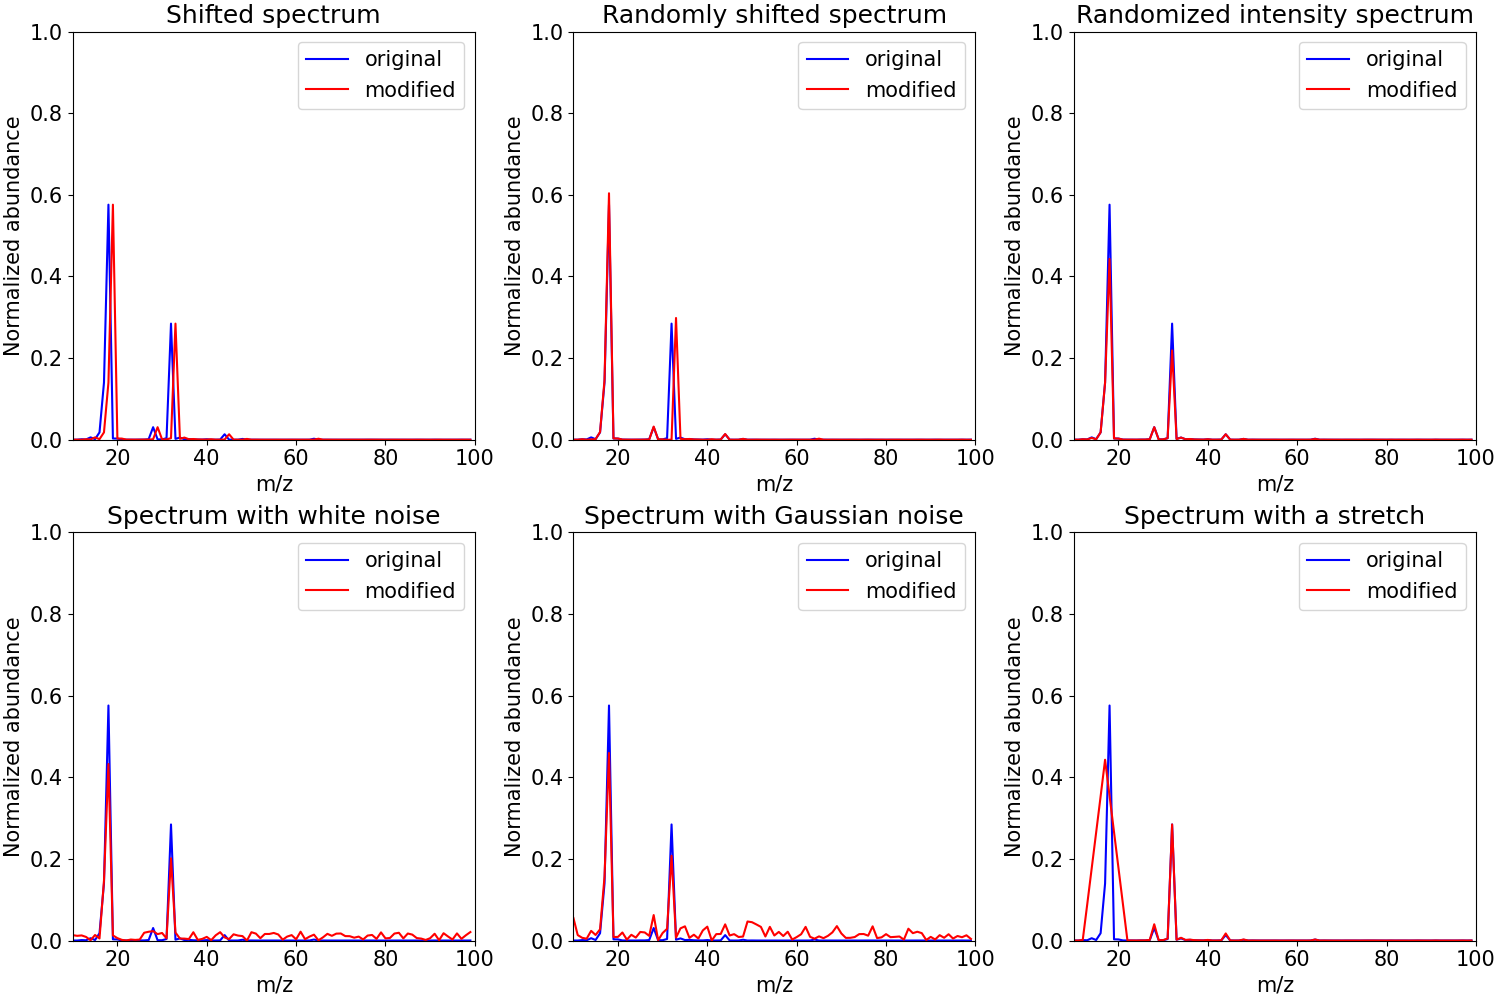
\includegraphics[width=1\linewidth]{chapter8/figs/data_aug3.png}
    \caption{6 basic data augmentations on a single spectrum of a mass spectrometry sample}
    \label{fig:data-aug}
\end{figure}

\begin{figure}[h]
    \centering
    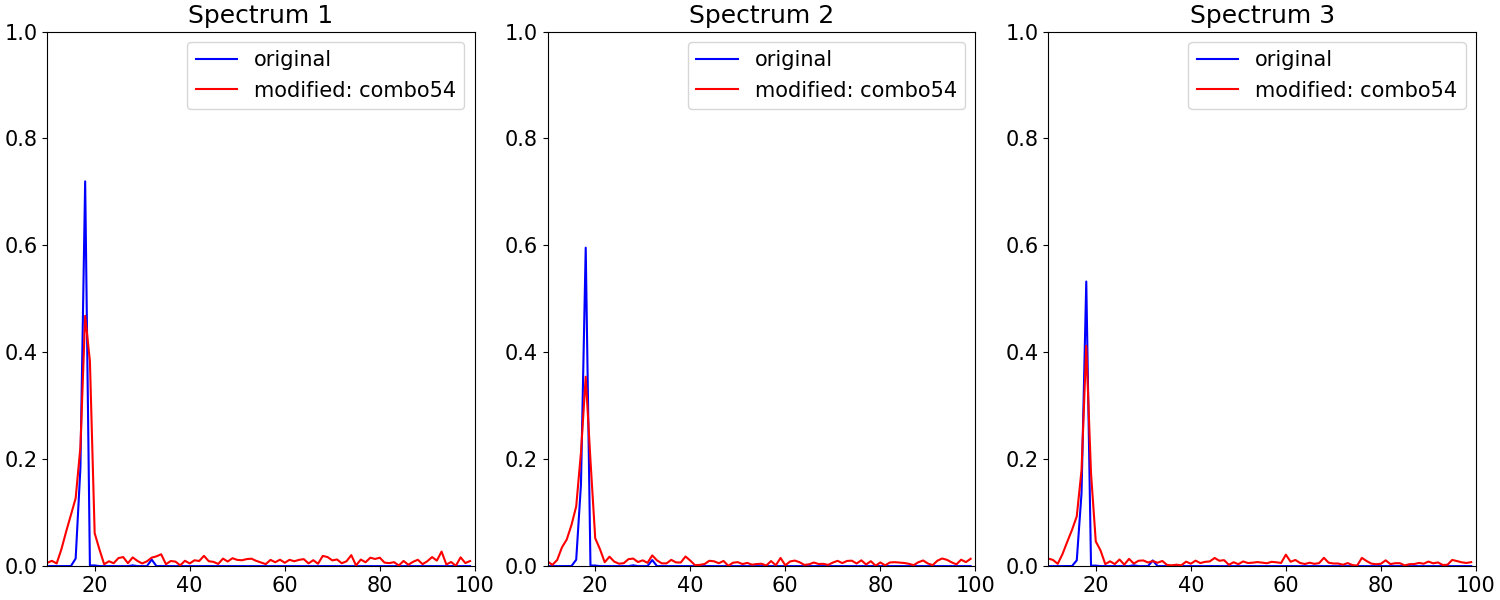
\includegraphics[width=1\linewidth]{chapter8/figs/data_aug_comb.png}
    \caption{One of the combinatorial data augmentations on three consecutive spectra of a single mass spectrometry sample}
    \label{fig:data-aug-comb}
\end{figure}


\subsection{Data Distributions and Outputs} \label{sec:data_outputs}

Following the completion of data preparation, the next step involves exploring data representations suitable for ML applications. One caveat is the limited amount of data; however, this limitation offers the advantage of enabling the implementation and testing of various ML approaches within a short timescale. Thus, numeric, image, and video-based outputs were generated for the entire dataset. The numeric data were represented as stacked 2D arrays for each sample, the image was represented as waterfall plots, and the video representation followed the format discussed in section 4. For both the video and image representations, axis markers and axis labels were omitted.

As outlined in section 5, data augmentation became necessary before developing ML algorithms. Consequently, as discussed in the section 5, both datasets increased in size by a factor of 64. The data was then split into training and test sets. Specifically, 85\% of the samples from the commercial data are used to train the model, with the remaining 15\% representing the test data set. Since the "Nitrate" label is not present in the commercial samples, roughly half of the SAM samples containing "Nitrate" are added to the training set, and all remaining SAM samples constitute the test set used for model validation. During the sample division, it is also ensured that the distribution of the percentage of chemical signatures is similar between the training and test sets. The exact distribution of the data and associated labels is presented in \cref{fig:train_test_split}.

\begin{figure}[h]
    \centering
    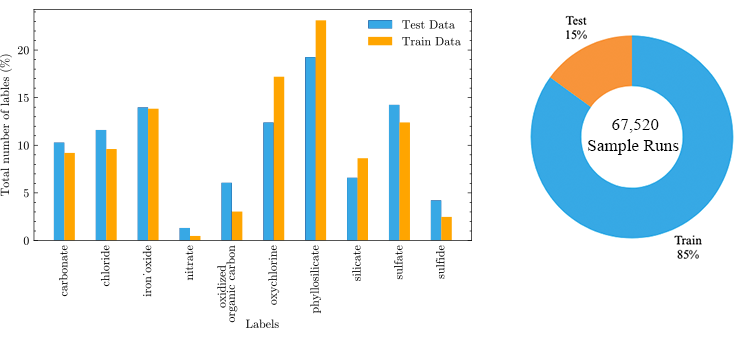
\includegraphics[width=0.9\linewidth]{chapter8/figs/train_test_split.png}
    \caption{\textit{Left} Distribution of labels as a function of total percentage. \textit{Right} Distribution of test and training split of the data. }
    \label{fig:train_test_split}
\end{figure}

\subsection{Supervised Machine Learning Methods}

Machine learning (ML) techniques are used to identify the patterns in mass spectral peak variations with temperature (time) corresponding to different chemical compounds. Since the identification of chemical compounds occurs at the end of a sample run, multiple labels are associated with a sample experiment. This corresponds to a multi-label multi-class classification ML problem, and both supervised and semi-supervised techniques are explored to investigate this problem.

\subsection{Supervised Learning} \label{sec:supervised}
Supervised learning techniques are also used, which involve labeled mass spectral data being used to train a model and make label predictions on unknown mass spectral data. An important deciding factor for the employed supervised learning technique is the input type of the spectral data---tabular/array, image, or video. The tabular-data-based classical supervised models and image-based convolutional neural network (CNN) models are examined below, and the video-based CNN networks are discussed in the section \ref{sec:discussions}.

The performance of all the models is evaluated using standard metrics such as precision and recall, and additionally using specificity and fall out for the image-based CNN network. The mathematical expression for these metrics is:
\begin{equation}
    \begin{split}
        \text{Precision} = \left( \frac{\text {TP}}{\text {TP + FP}} \right), \quad  \text{Recall}    = \left( \frac{\text {TP}}{\text {TP + FN}} \right), \\
        \text{Specificity} = \left( \frac{\text {TN}}{\text {TN + FP}} \right) \quad  \text{Fall out} = \left( \frac{\text {FP}}{\text {TN + FP}} \right)
    \end{split}
\end{equation}
Here, both precision and recall measure the quality of correct positive predictions. High precision indicates fewer false positives, while high recall indicates fewer false negatives. On the other hand, specificity and fallout assess the quality of negative predictions. Higher specificity suggests that the model correctly predicts more true negatives, whereas higher fallout indicates that the model misclassifies more negative data points. A model that performs well is characterized by high values of precision, recall, and specificity, and low values of fallout.

\subsubsection{Classical Classification ML Models}

As various chemical compounds labels can be present in a single sample, multi-label classifiers need to be employed. In this several multi-label classification algorithms are explored. 
These included Random Forest and Decision Trees algorithms. These models are well-suited for handling the interdependencies among the labels, which enable the capture of complex relationships between mass spectral peaks and corresponding chemical compound. 
Using numeric data input as described in \cref{sec:data_outputs}, each model was deployed using the CPU based \texttt{scikitlearn}. The results of each classifier are presented in \cref{tab:sckitlearn_results}. \\


\begin{table}[]
  \centering
  \footnotesize
  \begin{tabular}{|l||*{4}{c|}}\hline
    \backslashbox{Label}{Model} & \multicolumn{2}{c|}{\textbf{Decision trees}} & \multicolumn{2}{c|}{\textbf{Random Forest}} \\\hline
    & Precision & Recall & Precision & Recall \\\hline\hline
    Carbonate & 0.71 & 0.74 &  0.76 & 0.67 \\
    Chloride & 0.60 & 0.57 &  0.83 &  0.66 \\
    Iron oxide  & 0.81 & 0.57  & 0.94 & 0.55 \\
    Nitrate  & 0.27 & 0.80 &  0.24 & 0.78 \\
    Oxidized organic carbon & 0.79 & 0.96 & 0.87 & 0.57 \\ 
    Oxychlorine & 0.67 & 0.74 & 0.70 & 0.81 \\ 
    Phyllosilicate & 0.81 & 0.66 & 0.89 & 0.55 \\
    Silicate & 0.43 & 0.52  & 0.94 & 0.68 \\
    Sulfate & 0.69 & 0.63 &  0.83 & 0.83 \\ 
    Sulfide & 0.42 & 0.50 &  0.44 & 0.44 \\
    \hline
  \end{tabular}
  \caption{Precision and Recall for each label in classical ML classifiers employed in this study.} 
  \label{tab:sckitlearn_results}
\end{table}




\subsubsection{Image-based CNN Model}
Convolutional Neural Networks (CNN) are traditionally known to perform well for classification problems on input images (e.g., \cite{guo2017simple,elngar2021image}). Here, we represent sample runs as images such that each pixel in the image corresponds to a normalized abundance for an m/z value at a particular time (see Fig \ref{fig:2dd-cnn}). We base our model on pre-trained ResNet (Residual Networks) \citep{he2016deep} and modify the last activation and loss function to use sigmoid function and binary-cross-entropy loss, respectively, to allow for multi-label image classification.  \\

We test our implementation using the available PyTorch Image Models (through module \texttt{timm}) and find good fits with models based on 50-layers, i.e., ResNet50, ResNet50\_v2 and ResNet50\_gn.  Our best-fitting model, ResNet50\_gn, gives $68 \%$ accuracy comparing all the predicted labels with the test labels. However, the accuracy computed based on whether a given label is present or not is much better (close to 90\% for all labels, table \ref{table:metrics_image_cnn}). All these models were run one A100 NVIDIA GPU and took two to four hours to train approximately 55,000 images.

\begin{figure}
    \centering
    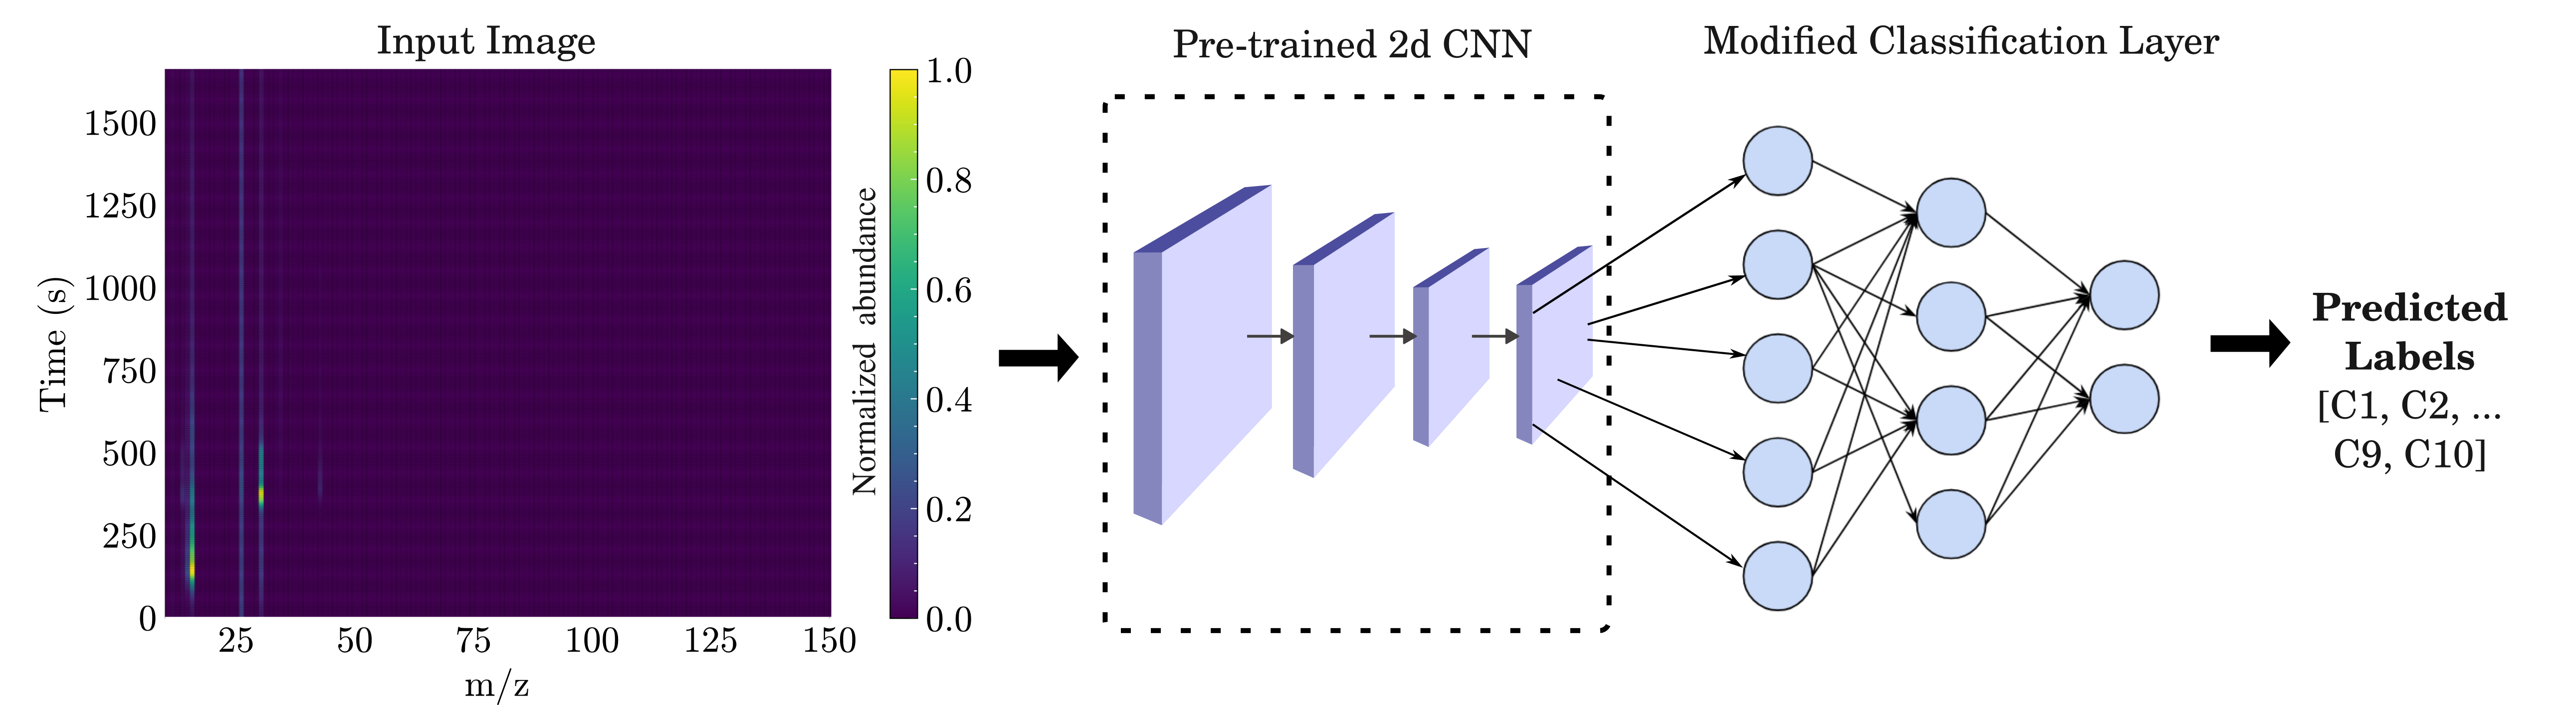
\includegraphics[width=\linewidth]{chapter8/figs/Image-cnn.png}
    \caption{Schematic of the image-based CNN network that takes input spectral data to classify the constituent chemical signatures. The input images are first passed through the pre-trained layers in the network and then through the modified last layer for classification. The input image represents the normalized abundance with mass over charge and time through the sample run.}
    \label{fig:2dd-cnn}
\end{figure}



\begin{table}[h!]
\centering
 \footnotesize
\begin{tabular}{||c| c c c c||} 
 \hline
 \textbf{Label} &  \textbf{Precision} & \textbf{Recall} & \textbf{Specificity} & \textbf{Fall out}\\ [0.5ex] 
 \hline\hline
 Carbonate & 0.89& 0.90 & 0.95 & 0.0458 \\ 
 Chloride & 0.91 & 0.91 &  0.97 & 0.0317 \\
 Iron oxide  & 0.86 & 0.86  & 0.96 & 0.0423\\
 Nitrate  & 0.98 & 0.93 & 0.93 & 0.0720 \\
 Oxidized organic carbon & 0.93 & 0.93 & 0.97 & 0.0280 \\ 
 Oxychlorine & 0.88 & 0.85 & 0.85 & 0.1520 \\ 
 Phyllosilicate & 0.84 & 0.84 & 0.93 & 0.0710  \\
 Silicate$^*$ & 0.95 & 0.95 & 0.98 & 0.0205 \\
 Sulfate & 0.90 & 0.90 & 0.94 & 0.0560 \\ 
 Sulfide & 0.90 & 0.88 &  0.92 & 0.0832 \\ [1ex] 
 \hline
\end{tabular}
\caption{Performance metrics for each label in the Resnet50\_gn model. $^*$The compound that the model identifies most reliably.}
\label{table:metrics_image_cnn}
\end{table}

\section{Discussion} \label{sec:discussions}
The results presented in \cref{tab:sckitlearn_results} demonstrate that Random Forest generally outperforms Decision Trees in both precision and recall across most labels, which is expected given the ensemble nature of Random Forests that reduce overfitting and improve generalization. For instance, the precision for the iron oxide label is significantly higher in Random Forest (0.94) compared to Decision Trees (0.81), indicating better discrimination of true positives. However, specific labels like Nitrate show high recall but low precision with Decision Trees, suggesting a high false-positive rate, possibly due to lack of enough Nitrate samples as they are only present in the Mars dataset. Labels such as Chloride benefit considerably from the Random Forest's improved precision (0.83 vs. 0.60 in Decision Trees), highlighting its superior performance in cases where Decision Trees struggle. The variance in model performance across different labels may also point to potential challenges such as complexity of distinguishing certain classes. Moving forward, these results suggest the need for further hyperparameter tuning or feature engineering to enhance classification accuracy, particularly for labels where significant disparities exist between models. \\

The image-based CNN network can classify most of the chemical signatures with approximately 90\% confidence (see Table \ref{table:metrics_image_cnn}). The compound best identified using this network is Silicate, which has around 95\% precision and recall and low fallout values. This suggests that Silicate is most distinctly isolated in the time and abundance space compared to the other chemical compounds. Conversely, Oxychlorine is the most challenging to classify using this CNN network. This could be due to spectral mixing---peaks occurring at m/z values very close to each other---of Chlorine (atomic mass 17) and Oxygen-bearing (atomic mass 16) compounds. \\


Based on the results from these models, future directions to improve the models performance are discussed in \cref{subsec:way-forward}. In addition to the models presented above, several other models were explored that are summarized in \cref{subsec:unsucessful_models}. 

\subsection{Immediate Way Forward}\label{subsec:way-forward}

The varying results for identifying a chemical compounds in the classical ML classifiers (see \ref{subsec:semi-supervised}), point to the different capabilities of each of the two models. Therefore, exploring other ensemble methods like Gradient Boosting could provide further improvements. Ultimately, the choice between models may depend on the application context, where different trade-offs between precision and recall are necessary, such as favoring models with higher recall for cases where false negatives are particularly costly.\\ The preferred step forward would be testing more classifiers and combining the advantages of each classifier in an ensemble configuration maximising individual label accuracy.\\ From our preliminary analysis with bootstrapping and averaging of the models' results, no improvement over the 2D-CNN network was found, and therefore a more careful implementation of an ensemble model is needed.\\
The next step to enhance the robustness of our ML models involves applying the clustering algorithm (as discussed in Section \ref{subsec:semi-supervised}) to all Mars samples. This will help  identify intermediate spectra labels and potentially uncover any missing labels. By incorporating the labeled spectra obtained from the clustering process into our ML models, it can be assessed whether this additional information improves their performance. \\

The performance of our models can also be tested on a different MS dataset. Similar to EGA, data from Gas Chromatography Mass Spectrometer (GCMS) from SAM and commercial instruments is publicly hosted by NASA's MSL PDS archive. The GCMS data, which involves longer sample runs and a different set of chemical signatures compared to EGA, is considered a valuable dataset. The same data pre-processing and augmentation techniques used for the EGA dataset will be applied to the GCMS data, and the performance of our models with this new dataset will be evaluated. 


\subsection{Unsuccessful Models} \label{subsec:unsucessful_models}
The image-based CNN models that provide a good predictions are all based on ResNet50. However, we note that other adaptions of ResNet networks did not perform as well. In particular, ResNet10, ResNet14t, ResNet18, ResNet26, ResNet34, and ResNet101 were not able to make accurate label predictions. The better performance of Resnet50 has also been observed in other studies for image classification (e.g., \citet{sharma2018analysis}, \citet{reddy2019transfer}, \citet{shabbir2021satellite} etc.), validating its architecture for transfer learning---a technique in which a trained model on one dataset is adapted to perform a different dataset---applications. A likely explanation for the better performance of ResNet50-based models could be that these models can offer a good balance between the complexity of the problem and the risk of overfitting the dataset. \\

A natural choice for time-series data is Recurrent Neural Networks (RNNs) and Long Short-Term Memory networks (LSTMs). We use three layers in RNN: an embedding layer(to ensure that the sizes are same from the input array for input into a model), RNN model layer with varying hidden units, and a fully connected layer that transforms the model to an output classification vector. Since LSTMs do not require a fixed input size, we use one layer for the model and one fully connected layer to the output layer for classification.  In our preliminary analysis using shallow RNNs and LSTMs, it was observed that the models' accuracy did not increase and the loss did not decrease with increasing epochs. It was also observed that due to the complex architecture of LSTM networks, a limitation was imposed by CUDA memory on our GPU, restricting batch sizes to up to 4. The results remained unchanged even when various batch sizes and loss functions were tested. One possible reason for this is that zero-padding was used to handle different time-sequence lengths in the data, ensuring that each batch had sequences of the same length. It is suggested that this zero-padding might have affected the model’s performance by drowning the signal in the data. This issue can be mitigated in the future by using more robust techniques for padding, such as interpolating the gaps using the last known non-zero intensity value to ensure information continuity.
% missing time using optical flow. \\

The performance of a video-based CNN network was also investigated, with the model implementation being similar to that of an action-based CNN network. As with the RNNs, improvements in accuracy with increasing epochs were not found. One possible explanation for this could be that meaningful patterns are not learned by these models, as the time-evolution of the spectra is somewhat too simple. In other words, significant changes in the evolution of spectral peaks do not occur within the sample runs, making them difficult to be captured by this model. Another factor could be that only a portion of the total augmented dataset was used for training the model due to CUDA memory limitations, which prevented the use of the entire dataset of 55,000 videos.

\subsection{Roadmap for Future}
The objectives of this project are twofold: first, to create an ML model that accelerates the classification of chemical compounds from spectra for scientists on Earth, and second, to extend the model for in-situ deployment, enabling it to autonomously assess and make decisions on whether the sample is \textit{interesting} or not. Towards both of these goals, the ML models based on our analysis in this study are summarized in Table \ref{table:summary}.


\begin{table}[h!]
\centering
\begin{tabular}{|p{4 cm}|p{2.5 cm}|p{2.5 cm}|p{2.5 cm}|p{2.5 cm}|} 
 \hline
 \textbf{Criterion} & \textbf{Classical ML} &  \textbf{2D CNN} & \textbf{3D CNN} & \textbf{RNN/LSTM} \\ [0.5ex]
 \hline
 Ability for on-ground tool   & \checkmark & \checkmark & \checkmark & \checkmark \\
 Reliable predictions & \checkmark & \checkmark &  x  &  x \\
 CUDA memory efficient &  \checkmark & \checkmark &  x  &  x \\
 In-situ deployment &   \checkmark & \checkmark  &  x  &  x \\

\hline
\end{tabular}
\caption{Summary of models analyzed and their applicability in future space missions.}
\label{table:summary}
\end{table}

\section{Conclusions}
Machine learning models are employed to explore their effectiveness in classifying chemical compounds from MS data. Specifically, data from the SAM instrument aboard the Mars \textit{Curiosity} rover, as well as data from NASA's commercial instruments used in SAM's development, was utilized in this FDL challenge. To address the challenge of insufficient data (around 1,700 sample runs) for training the ML models, various data augmentation techniques are applied to create synthetic data that is both scientifically accurate and consistent with the original spectral behavior.

Among the ML models evaluated, ResNet50\_gn, a pre-trained 2D CNN, was the most effective. Although this model was trained on a large and diverse dataset unrelated to the specific spectral images, its performance suggests that transfer learning could be a valuable approach for classifying MS data into chemical compounds. This model achieved over 84\% precision and recall for all identified chemical compounds, with precision and recall reaching up to 94\% for some compounds. \\ Good fits were also obtained with the classical ML classifiers. Between the two methods explored—Random Forest and Decision Trees—better fits were achieved with the Random Forest classifier. Specifically, the Random Forest classifier achieved over 80\% precision for most chemical compounds and up to 94\% for silicates. The recall values for these compounds were somewhat lower, between 65\% and 80\%, indicating some difficulty in uniquely classifying these compounds using classical methods. An ensemble method that combines the strengths of different classifiers could potentially improve the prediction accuracy of classical methods.

To further improve the performance and validate the robustness of the models tested, several short-term tasks are proposed. However, this analysis is considered an initial step toward the development of an in-situ classification model, and further investigation is required to achieve a fully autonomous classifier.